%% Stellarium User Guide

\chapter{Deep-Sky Objects}
\label{ch:DSO}


Since version 0.10.0 Stellarium uses the ``json'' cataloguing system
of configuring textures. At the same time the Simbad online catalogue
was added to the search feature, making the catalog somewhat redundant
and used now only as a first search point or if there is no internet
connection.

If the object has a name (not just a catalogue number), you should add
one or more records to the \file{.../nebulae/default/names.dat} file
(where \file{...} is either the installation directory or the user
directory). See section~\ref{sec:dso:modifyingNamesDat} Modifying \file{names.dat}
for details of the file format.

If you wish to associate a texture (image) with the object, you must 
add a record to the \file{.../nebulae/default/textures.json} file. See
section~\ref{sec:dso:modifyingTexturesJson} for details of the file format.


\section{Stellarium DSO Catalog}
\label{sec:dso:catalog}

Stellarium's DSO Catalog contains over 85000 objects\footnote{An extended edition of this catalog 
with over one million objects may be downloaded and installed manually (see section \ref{sec:ExtraData:DSOs}).} 
(up to $15.5^m$) and is available for end users as collection of files:

\begin{longtabu} to \textwidth {lX}
%\emph{File} & \emph{Description}\\
\file{catalog.txt} &Stellarium DSO Catalog in ASCII format for editing data\\
\file{catalog.dat} &Stellarium DSO Catalog in zipped binary format for usage within Stellarium\\
\file{names.dat}   &List of proper names of the objects from file \file{catalog.dat}
\end{longtabu}

ASCII file can be converted into binary format through enabling an option in the file \file{config.ini} (See \ref{sec:ConfigurationFile}):
\begin{configfile}
[devel]
convert_dso_catalog = true
\end{configfile}

The file \file{catalog.txt} should be put into the directory
\file{.../nebulae/default/} and you should create an empty 
file \file{catalog.pack} to storing the binary catalog. 
After converting the data into binary format you should 
zipped them by command \command{gzip -nc catalog.pack > catalog.dat}.

Stellarium DSO Catalog contains data and supports the designations for
follow catalogues:

\begin{description}[align=right,labelwidth=2cm]
\item[\textbf{NGC}]  New General Catalogue 
\item[\textbf{IC}] Index Catalogue 
\item[\textbf{M}] Messier Catalog
\item[\textbf{C}] Caldwell Catalogue 
\item[\textbf{B}] Barnard Catalogue~\cite{1927cdos.book.....B} 
\item[\textbf{SH2}] Sharpless Catalogue~\cite{1959ApJS....4..257S} 
\item[\textbf{VdB}] Van den Bergh Catalogue of reflection nebulae~\cite{1966AJ.....71..990V} 
\item[\textbf{RCW}]  A catalogue of H$\alpha$-emission regions in the southern Milky Way~\cite{1960MNRAS.121..103R} 
\item[\textbf{LDN}]  Lynds' Catalogue of Dark Nebulae~\cite{1962ApJS....7....1L} 
\item[\textbf{LBN}]  Lynds' Catalogue of Bright Nebulae~\cite{1965ApJS...12..163L} 
\item[\textbf{Cr}] Collinder Catalogue~\cite{1931AnLun...2....1C} 
\item[\textbf{Mel}]  Melotte Catalogue of Deep Sky Objects~\cite{1915MmRAS..60..175M} 
\item[\textbf{PGC}]  HYPERLEDA. I. Catalog of galaxies\footnote{The PGC and UGC catalogues have a partial support}
\item[\textbf{UGC}]  The Uppsala General Catalogue of Galaxies
\item[\textbf{Ced}]  Cederblad Catalog of bright diffuse Galactic nebulae~\cite{1946MeLuS.119....1C}
\item[\textbf{Arp}]  Atlas of peculiar galaxies~\cite{1966ApJS...14....1A}\newFeature{V0.16.0}
\item[\textbf{VV}]  The catalogue of interacting galaxies by Vorontsov-Velyaminov~\cite{2001A&AT...20..717V}\newFeature{V0.16.0}
\item[\textbf{PK}]  Version 2000 of the Catalogue of Galactic Planetary Nebulae~\cite{2001A&A...378..843K}\newFeature{V0.16.0}
\item[\textbf{PN G}]  The Strasbourg-ESO Catalogue of Galactic Planetary Nebulae~\cite{1992secg.book.....A}\newFeature{V0.16.1}
\item[\textbf{SNR G}]  A catalogue of Galactic supernova remnants~\cite{2014yCat.7272....0G}\newFeature{V0.16.1}
\end{description}

Cross-index data for Stellarium DSO Catalog is partially obtained from ``Merged catalogue of reflection nebulae''~\cite{2003A&A...399..141M} and astronomical databases SIMBAD\footnote{SIMBAD Astronomical Database --- \url{http://simbad.u-strasbg.fr/simbad/}}~\cite{2000A&AS..143....9W} and NED\footnote{NASA/IPAC Extragalactic Database (NED) --- \url{https://ned.ipac.caltech.edu/}}.

\subsection{Modifying catalog.dat}
\label{sec:dso:modifyingCatalog.dat}

This section describes the inner structure of the files \file{catalog.dat}
(binary format) and \file{catalog.txt} (ASCII format).
Stellarium can convert ASCII file into the binary format file for faster usage
within the program.

Each line contains one record, each record consisting of the following
fields with \emph{tab} char as delimiter:

\begin{longtabu} to \textwidth {l|l|X}
\toprule
\emph{Column} & \emph{Type} & \emph{Description}\\\midrule
 1 & integer & Deep-Sky Object Identificator\\
 2 & float   & RA (decimal degrees)\\
 3 & float   & Dec (decimal degrees)\\
 4 & float   & B magnitude\\
 5 & float   & V magnitude\\
 6 & string  & Object type (See section~\ref{sec:dso:types} for details).\\
 7 & string  & Morphological type of object\\
 8 & float   & Major axis size or radius (arcmin)\\
 9 & float   & Minor axis size (arcmin)\\
10 & integer & Orientation angle (degrees)\\
11 & float   & Redshift\\
12 & float   & Error of redshift\\
13 & float   & Parallax (mas)\\
14 & float   & Error of parallax (mas)\\
15 & float   & Non-redshift distance (\Mpc\ for galaxies, \kpc\ for other objects)\\
16 & float   & Error of non-redsift distance (\Mpc\ for galaxies, \kpc\ for other objects)\\
17 & integer & NGC number (New General Catalogue)\\
18 & integer & IC number (Index Catalogue)\\
19 & integer & M number (Messier Catalog)\\
20 & integer & C number (Caldwell Catalogue)\\
21 & integer & B number (Barnard Catalogue)\\
22 & integer & SH2 number (Sharpless Catalogue)\\
23 & integer & VdB number (van den Bergh Catalogue of reflection nebulae)\\
24 & integer & RCW number (A catalogue of H$\alpha$-emission regions in the southern Milky Way)\\
25 & integer & LDN number (Lynds' Catalogue of Dark Nebulae)\\
26 & integer & LBN number (Lynds' Catalogue of Bright Nebulae)\\
27 & integer & Cr  number (Collinder Catalogue)\\
28 & integer & Mel number (Melotte Catalogue of Deep Sky Objects)\\
29 & integer & PGC number (HYPERLEDA. I. Catalog of galaxies); partial\\
30 & integer & UGC number (The Uppsala General Catalogue of Galaxies); partial\\
31 & string  & Ced number (Cederblad Catalog of bright diffuse Galactic nebulae)\\
32 & integer & Arp number (Atlas of Peculiar Galaxies)\\
33 & integer & VV number (The catalogue of interacting galaxies)\\
34 & string  & PK identificator (Catalogue of Galactic Planetary Nebulae)\\
35 & string  & PN G identificator (The Strasbourg-ESO Catalogue of Galactic Planetary Nebulae)\\
36 & string  & SNR G identificator (A catalogue of Galactic supernova remnants)\\
\bottomrule
\end{longtabu}

\subsubsection{Types of Objects}
\label{sec:dso:types}

Possible values for type of objects in the file \texttt{catalog.dat}.

\begin{longtabu} to \textwidth {l|X}
\toprule
\emph{Type} & \emph{Description}\\\midrule
G   & Galaxy\\
GX  & Galaxy\\
AGX & Active Galaxy\\
RG  & Radio Galaxy\\
IG  & Interacting Galaxy\\
GC  & Globular Cluster\\
OC  & Open Cluster\\
NB  & Nebula\\
PN  & Planetary Nebula\\
DN  & Dark Nebula\\
RN  & Reflection Nebula\\
C+N & Cluster associated with nebulosity\\
HII & HII Region\\
SNR & Supernova Remnant\\
SNC & Supernova Candidate\\
SNRC & Supernova Remnant Candidate\\
BN  & Bipolar Nebula\\
EN  & Emission Nebula\\
SA  & Stellar Association\\
SC  & Star Cloud\\
CL  & Cluster\\
IR  & Infra-Red Object\\
QSO & Quasar\\
Q?  & Possible Quasar\\
ISM & Interstellar Matter\\
EMO & Emission Object\\
LIN & LINEAR-type Active Galaxies\\
BLL & BL Lac Object\\
BLA & Blazar\\
MOC & Molecular Cloud\\
YSO & Young Stellar Object\\
PN? & Possible Planetary Nebula\\
PPN & Protoplanetary Nebula\\
$\ast$ & Star\\
$\ast\ast$ & Double Star\\
MUL & Multiple Star\\
SY$\ast$ & Symbiotic Star\\
EM$\ast$ & Emission-line Star\\
\emph{empty} & Unknown type, catalog errors, \emph{Unidentified Southern Objects} etc.\\
\bottomrule
\end{longtabu}

\subsection{Modifying names.dat}%\label{modifying-names.dat}
\label{sec:dso:modifyingNamesDat}

Each line in the file \file{names.dat}  contains one record. A record
relates an extended object catalogue number (from \file{catalog.dat})
with a name. A single catalogue number may have more than one record in
this file.

The record structure is as follows:

\begin{longtabu} to \textwidth {l|l|l|X}
\toprule
\emph{Offset} & \emph{Length} & \emph{Type} & \emph{Description}\\
\midrule
0  &  5 & \%5s & Designator for catalogue (prefix)\\
5  & 15 & \%d  & Identificator for object in the catalog\\
20 & 60 & \%s  & Proper name of the object (translatable)\\
\bottomrule
\end{longtabu}

If an object has more than one record in the file \file{names.dat},
the last record in the file will be used for the nebula label.

\subsection{Modifying textures.json}%\label{modifying-textures.json}
\label{sec:dso:modifyingTexturesJson}

This file is used to describe each nebula image. The file structure
follows the JSON format, a detailed description of which may be found
at \url{www.json.org}. The \file{textures.json} file which ships with
Stellarium has the following structure:

%% TODO: GZ notes 2016-04 It seems there is some overdocumentation here, some entries seem to repeat in this list. FIX THAT!

\begin{description}
\item[serverCredits (optional)] a structure containing the following
  key/value pairs:

  \begin{description}
  \item[short] a short identifier of a server where the json file is found, e.g. ``ESO''
  \item[full]  a longer description of a server, e.g. ``ESO Online Digitised Sky Survey Server''
  \item[infoURL] a URL pointing at a page with information about the server
  \end{description}
\item[imageCredits] a structure containing the same parts as a
  serverCredits structure but referring to the image data itself
\item[shortName] an identifier for the set of images, to be used inside Stellarium
\item[minResolution] minimum resolution, applies to all images in the set,
  unless otherwise specified at the image level
\item[maxBrightness] the maximum brightness of an image, applies to all
  images in the set, unless otherwise specified at the image level
\item[subTiles] a list of structures describing indiviual image tiles, or
  referring to another json file. Each subTile may contain:

  \begin{description}
  \item[minResolution]
  \item[maxBrightness]
  \item[worldCoords]
  \item[subTiles]
  \item[imageCredits]
  \item[imageUrl]
  \item[textureCoords]
  \end{description}
\item[shortName] (name for the whole set of images, e.g. ``Nebulae'')
\item[miniResolution] (applies to all images in set)
\item[alphaBlend] (applies to all images in set)
\item[subTiles] list of images. Each image record has the following properties:

  \begin{description}
  \item[imageCredits] (itself a list of key/pairs)
  \item[imageUrl] (e.g. file name)
  \item[worldCoords] (a list of four pairs of coordinates representing the corners of the image)
  \item[textureCoords] (a list of four pairs of corner descriptions. i.e. which is top left of image etc)
  \item[minResolution] (over-rides file-level setting)
  \item[maxBrightness]
  \end{description}
\end{description}

Items enclosed in Quotation marks are strings for use in the program.
Syntax is extremely important. Look at the file with a text editor to
see the format. Items in \textless{}\textgreater{} are user provided
strings and values to suit the texture and source.

\begin{configfile}[\footnotesize]
{
  "imageCredits"  : { "short" : "<author name>" , 
                      "infoUrl" : "http://<mysite.org>" 
                    }, 
  "imageUrl"      : "<myPhoto.png>",
  "worldCoords"   : [[[ X0, Y0], [ X1, Y1], [ X2, Y2], [ X3, Y3] ]], 
  "textureCoords" : [[[ 0,0],[1,0],[1,1],[0,1]]], 
  "MinResolution" : 0.2148810463,
  "maxBrightness" : <mag>
},
\end{configfile}

where 

\begin{description}
\item[worldCoords] Decimal numerical values of the J2000 coordinates (RA and dec both in degrees) of the corners of the texture. These values are usually given to 4 decimal places.
\item[textureCoords]  Where 0,0 is South Left, 1,0 the South Right, 1,1 North Right, 0,1 North Left corners of the texture.
\item[MinResolution] UNDOCUMENTED VALUE! Sorry!%% TODO FIXME!
\item[maxBrightness] total object brightness, magnitude 
\end{description}


Calculating of the coords of the corners of the images (plate solving) is
a time consuming project and needs to be fine tuned from the screen
display. As most images will be two dimensional, display on a spherical
display will limit the size to about 1 degree before distortion becomes
evident. Larger images should be sectioned into a mosaic of smaller
textures for a more accurate display.

\section{Adding Extra Nebulae Images}%\label{adding-extra-nebulae-images}
\label{sec:dso:adding_images}
\sectionauthor*{Barry Gerdes}

\subsection{\texorpdfstring{Preparing a photo for inclusion to the \file{textures.json} file}{Preparing a photo for inclusion to the textures.json file}}
\label{sec:dso:preparing-a-photo}

\begin{figure}[h]
\centering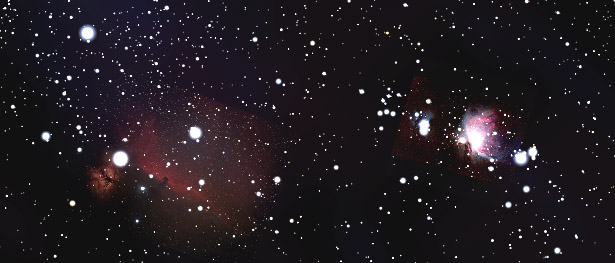
\includegraphics[width=\textwidth]{nebula-display}
\caption{Screen shot of nebula images displayed in Stellarium}
\label{fig:dso:preparing-a-photo}
\end{figure}

The first step is to take a photo of the object you wish to display in
Stellarium. When you have the picture you will need to align it with
the equatorial coordinate system so that north is directly up and not
inverted side to side or up and down as can happen with photos taken
with a diagonal mirror in the path. Next you will need to crop the
picture, setting the main feature at the centre and making the cropped
size a factor of $2^n$ eg. 64, 128, 256, 512, 1024 or 2048 pixels
square (or elongated like 512x1024).  If this requirement is not met,
your textures may not be visible, or graphics performance may be
seriously impacted. Textures larger than 2048 may only be supported on
high-end hardware. Images must be in PNG format.  When cropping, make
sure you leave at least six prominent background stars.

The next step is to process your photo to make the background
black, really black. This will ensure that your background will meld with the
Stellarium background and not be noticed as gray square. Suitable programs to do all
this are \program{The GIMP}\footnote{free in keeping with the Stellarium spirit; available from \url{http://www.gimp.org}} or
\program{Photoshop} if you can afford it.

When you have your image prepared you will need to plate solve it using
at least 6 known GSC stars that can be identified. That is why the
cropping with plenty of stars was necessary. When the plate is solved
you will need to find the J2000 coordinates of the corners and convert
them to decimal values to form the world coordinates in the
\file{textures.json} file.

\begin{figure}[htb]
\centering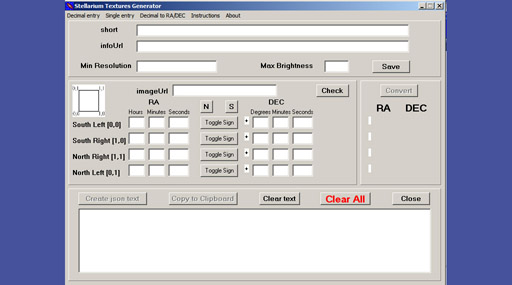
\includegraphics[width=\textwidth]{EQ-Decimal.jpg}
\caption{\program{Stellarium Textures Generator}: A program to convert Equatorial coordinates into decimal
form and write a \texttt{textures.json} insert}
\label{fig:dso:STGen}
\end{figure}

The program \program{Stellarium Textures Generator} by Peter Vasey (Fig.~\ref{fig:dso:STGen}) can convert the corner coordinates of a
texture found in your plate solving program into decimal values and write an
insert for the \file{textures.json} file.\footnote{It is available as a freebee
from
\url{http://www.madpc.co.uk/~peterv/astroplover/equipnbits/Stellariumtextures.zip}.}

\begin{figure}[ht]
\centering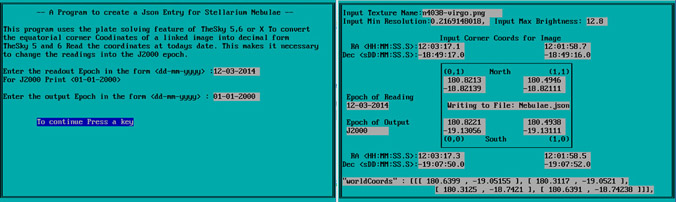
\includegraphics[width=\textwidth]{pix-4.jpg}
\caption{\program{ReadDSS}: A program to write a \file{textures.json} insert with epoch manipulation.}
\label{fig:dso:ReadDSS}
\end{figure}

There is another program, \program{ReadDSS} (Fig.~\ref{fig:dso:ReadDSS}), written by Barry Gerdes in Qb64(gl), that will perform the same
task but allows manipulation of the epochs.\footnote{
\url{http://barry.sarcasmogerdes.com/stellarium/uploads/writejsoninsert.zip}}

\subsection{Plate Solving}%\label{plate-solving}
\label{sec:dso:plateSolving}

Suitable programs that can accept your picture and calculate its corner
coordinates are hard to find. I have only found one that suits our
purpose and it is another expensive planetarium program, \program{TheSky X Pro}.
However the older versions \program{TheSky 5} and \program{6 Pro} will also do the job if
suitably configured, although I could not solve the test program with 
\program{TheSky 6} that uses the same procedure as \program{TheSky 5}.

These programs have a link feature that can match your photo to the
selected area of the screen and superimpose it on the display with a box
around your photo provided it can match at least 6 stars from the GSC
that is included with the program. When this is fitted you can read the
corner coordinates of your texture in the Status bar by selecting them
with a mouse. \program{TheSky X} can read these coordinates in J2000 values and
uses textures in the FITS format, but the earlier programs only read the
coordinates of the current program date. To read the J2000 coordinates
it is necessary to re-start the program with the date set to 1-1-2000.

To add the picture to \program{TheSky 5} you need first make a mono 8 bit version
of the photo and place it on the clipboard. Run \program{TheSky} and centre on the
object centre. Look in the \menu{Tools} menu for the \menu{image} link and select
\menu{setup}. Tick \menu{show image frame} to put a frame around the image.

Paste the clipboard image on the display and use the zoom and position
controls to get it as close to the size and position as possible by
visually matching stars. Go to the menu again and click on \menu{link wizard}.
If you have been successful the window will show the number of stars
matched and the option to \menu{accept} or \menu{continue}. Accept and you will now
see all the matched stars have overlaid the picture. You can now read
off the corner coordinates from the status bar starting at the bottom
(south) left and continuing counterclockwise to the top (north) left.

\subsection{\texorpdfstring{Processing into a \texttt{textures.json} insert}{Processing into a textures.json insert}}%\label{processing-into-a-textures.json-insert}

Place your image in the \file{*.png} format in the
\file{.../nebulae/default/} folder. Ensure that the name matches the
\file{textures.json} entry.

Once you have the corner coordinates of your photo you can add them to
the decimal converter program and it will write an insert
\file{nebula.json} as a text file that you can paste directly into the
\file{textures.json} file that is in the \file{.../nebulae/default/}
folder.

Save the \file{textures.json} file with the new insert and run
Stellarium. Find the object in the \key{F3} Object selection window and slew to
it. Your image should be there and with a bit of luck it will nicely
overlay the stars in Stellarium. However this only rarely
happens, so a little bit of tweaking of the JSON \parameter{worldcoords} will be
needed to get a perfect match. Select equatorial mode (\guibutton{0.6}{bt_coord_type} or \keys{\ctrl+M}).
This will show the area with north up. Select each corner in sequence
and make small changes to the coordinates. Restart Stellarium each time
and check if you have moved into the right direction. Continue with each
corner until all the stars match. With a little bit of practice this
will be done in about 10 minutes.


%%% Local Variables: 
%%% mode: latex
%%% TeX-master: "guide"
%%% End: 
